% !TEX encoding = UTF-8 Unicode
% !TEX root = thesis-ex.tex

This section will discuss the jet fragmentation as measured by the ATLAS detector for \pbpb\ collisions at $\sqrtsnn = 5.02$ TeV \cite{PhysRevC.98.024908}.
While measurements of \RAA \cite{20151, Aad:2014bxa, Khachatryan:2016jfl} and asymmetry \cite{Aaboud:2017eww, Chatrchyan:2011sx, PhysRevLett.119.062301} describe how much energy is lost by the jet, fragmentation measurements describe the momentum distribution of particles associated to the jet.
These can be described as:

\begin{align}
\Dz = \frac{1}{\Njet} \frac{d\nch}{dz} \\
\Dpt = \frac{1}{\Njet} \frac{d\nch}{d\pt}
\end{align}
where $z = \pt \cos(\Delta R / \ptjet)$ and gives the charged-particle longitudinal momentum fraction relative to the jet.
Modifications to the fragmentation functions in \pbpb\ collisions can be evaluated by constructing the ratios $\Rdz = \Dz_{\rm Pb+Pb} / \Dz_{pp}$ and $\Rdpt = \Dpt_{\rm Pb+Pb} / \Dpt_{pp}$.
The \Dpt\ distribution is shown in Figure~\ref{fig:jetff_dpt}.
%This measurement is corrected for detector effects and unfolded to the particle level.
%This allows for comparisons to other measurements and theoretical models.

\begin{figure}[htbp]
\begin{center}
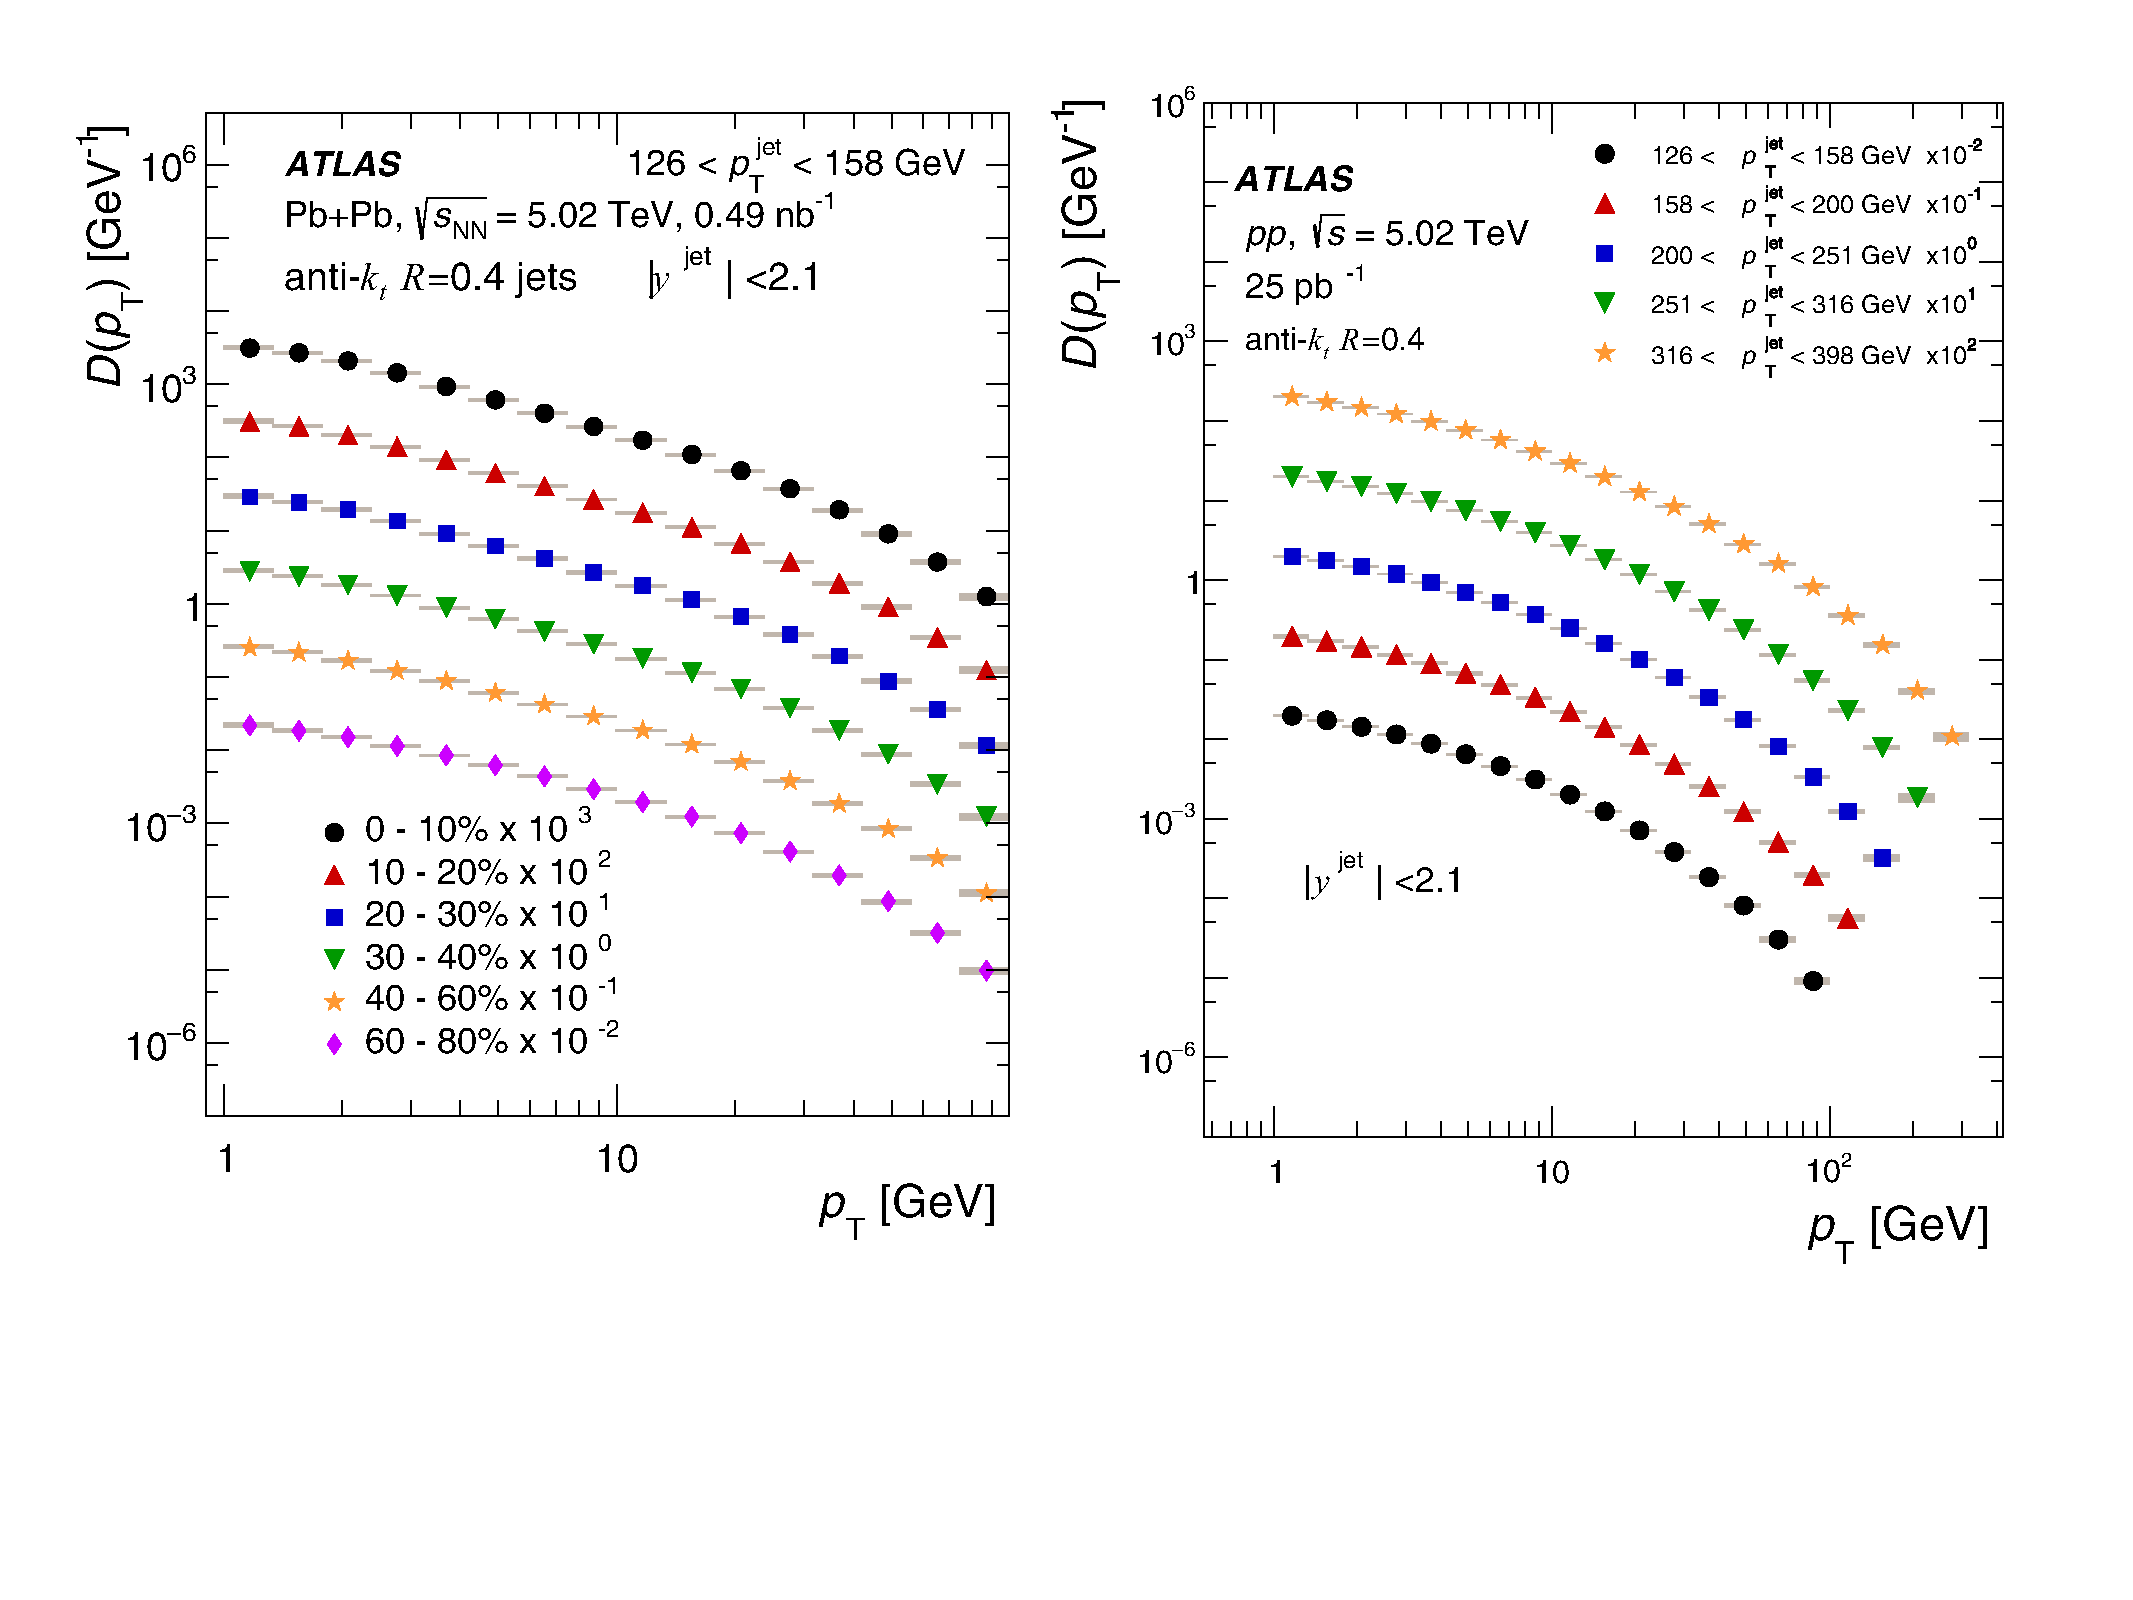
\includegraphics[width=0.65\textwidth]{figures/jetMeasurements/jetff_dpt}
\caption{(Left) The \Dpt\ distributions in \pp\ as a function of charged-particle \pt\ for different \ptjet\ selections and for jet rapidity $|y| < 2.1$.
(Right) The \Dpt\ distributions in \pbpb\ as a function of charged-particle \pt\ for different centrality selections and for jet rapidity $|y| < 2.1$.
The error bars represent statistical uncertainties while the shaded boxes represent systematic uncertainties.
Figure taken from \cite{PhysRevC.98.024908}.}
\label{fig:jetff_dpt}
\end{center}
\end{figure}


\begin{figure}[htbp]
\begin{center}
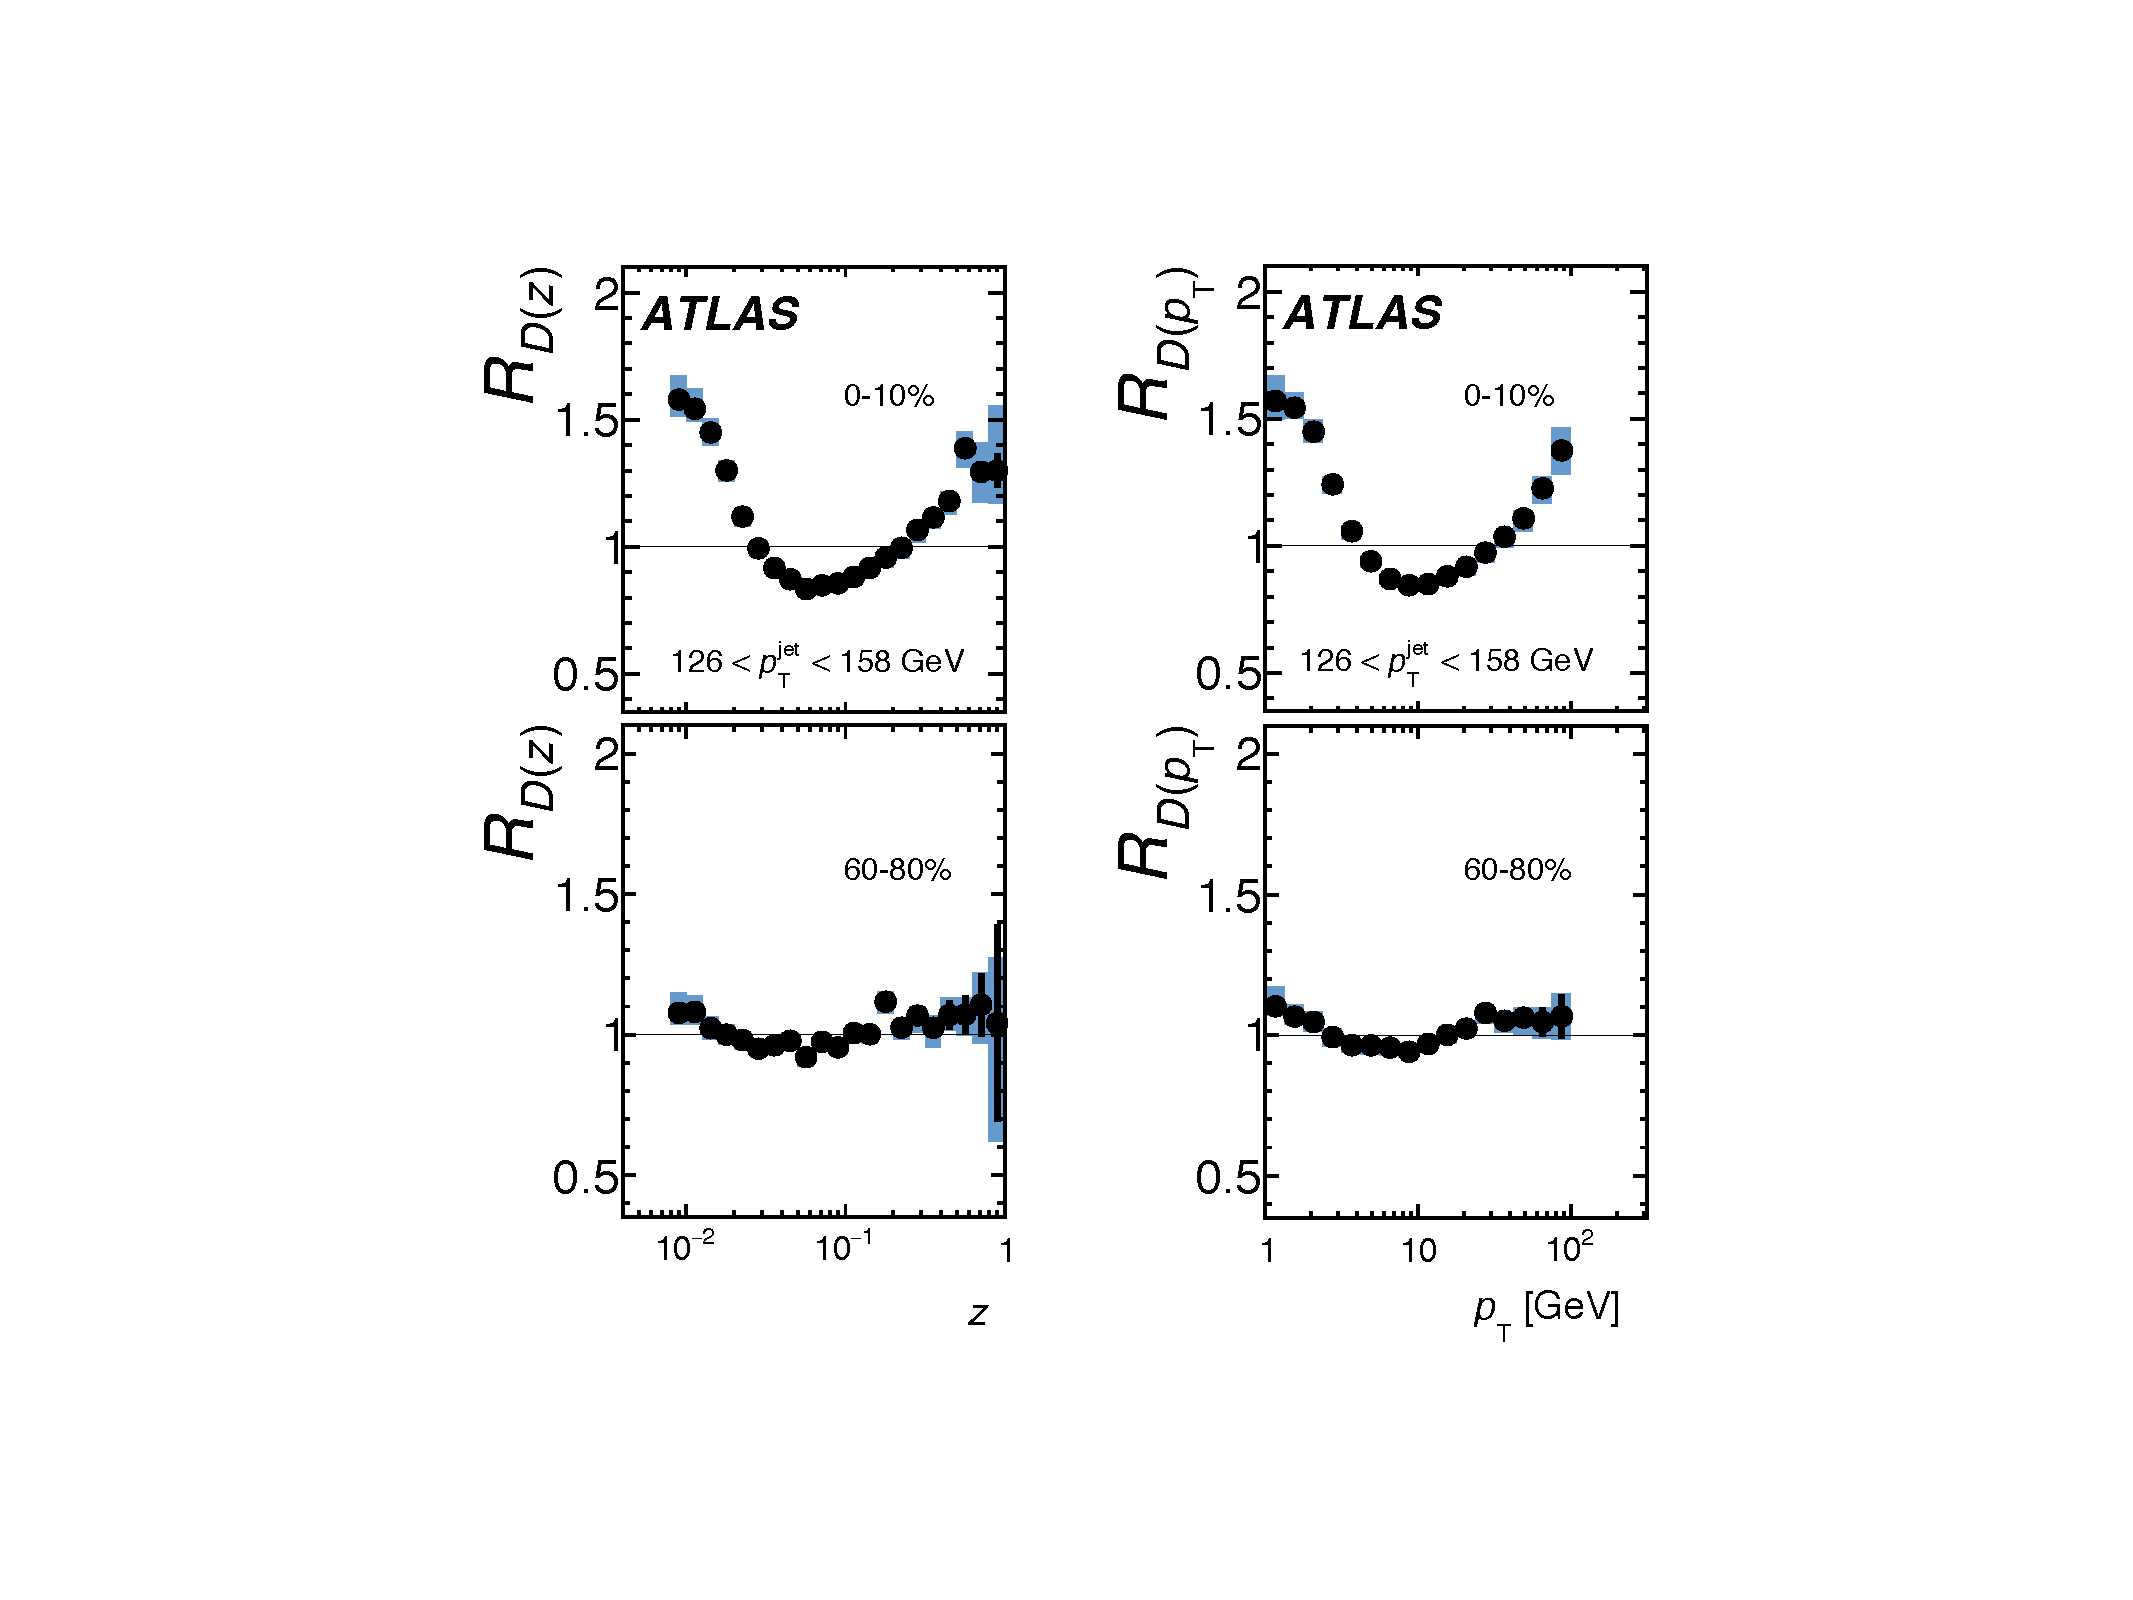
\includegraphics[width=0.65\textwidth]{figures/jetMeasurements/jetff_rdz_rdpt}
\caption{The modifications to the (left) \Dz\ and (right) \Dpt\ distributions in (top) 0--10\% central and (bottom) peripheral \pbpb\ compared to \pp\ as a function of charged-particle $z$ and \pt\ respectively.
The error bars represent statistical uncertainties while the shaded boxes represent systematic uncertainties.
Figures taken from \cite{PhysRevC.98.024908}.}
\label{fig:jetff_rdz_rdpt}
\end{center}
\end{figure}

The modifications to the \Dz\ and \Dpt\ distributions in central (top) and peripheral (bottom) collisions are shown in Figure~\ref{fig:jetff_rdz_rdpt}.
The shape of these modifications is very similar for both \Dz\ and \Dpt.
There is an enhancement of particles with low $z$ and \pt, followed by a suppression at intermediate $z$ and \pt, and finally an enhancement at high $z$ and \pt.
These modifications become smaller for more peripheral collisions.
The low momentum excess can be further investigated by calculating the extra number of particles \Nch\ in \pbpb\ compared to \pp\ as given below:

\begin{align}
\Nch = \int^{\pt_{\mathrm{max}}}_{\pt_{\mathrm{min}}} \left( \Dpt_{\pbpb} - \Dpt_{\pp} \right) d\pt
\end{align}
where $\pt_{\mathrm{min}} = 1$ GeV and $\pt_{\mathrm{max}} = 4.2$ GeV.

The \Nch\ distributions can be seen in Figure~\ref{fig:jetff_nch}.
It can be clearly seen that the size of the enhancement in \pp\ compared to \pp\ at low \pt\ increases as a function of \ptjet, growing from about 1.5 to 2.5 extra particles in the most central \pbpb\ collisions.
This excess is even seen in the peripheral \pbpb\ collisions, though it is a lot smaller and ranges from 0.2 to 0.5 extra particles.



%The \ptjet\ dependence of the \Rdz\ and \Rdpt\ distributions can be seen in Figure~\ref{fig:jetff_jetpt_dep}.
%This dependence can give insight into the modification of the fragmentation functions, with any scaling with $z$ indicating a change in the fragmentation pattern, while a scaling with \pt\ reflecting an effect from the medium itself.
%The low momentum excess in the \Rdpt\ distributions seen in Figure~\ref{fig:jetff_jetpt_dep} can be further studied by integrating over that region.
%Then the extra number of particles in \pbpb\ compared to \pp\ is given by:
%\begin{figure}[htbp]
%\begin{center}
%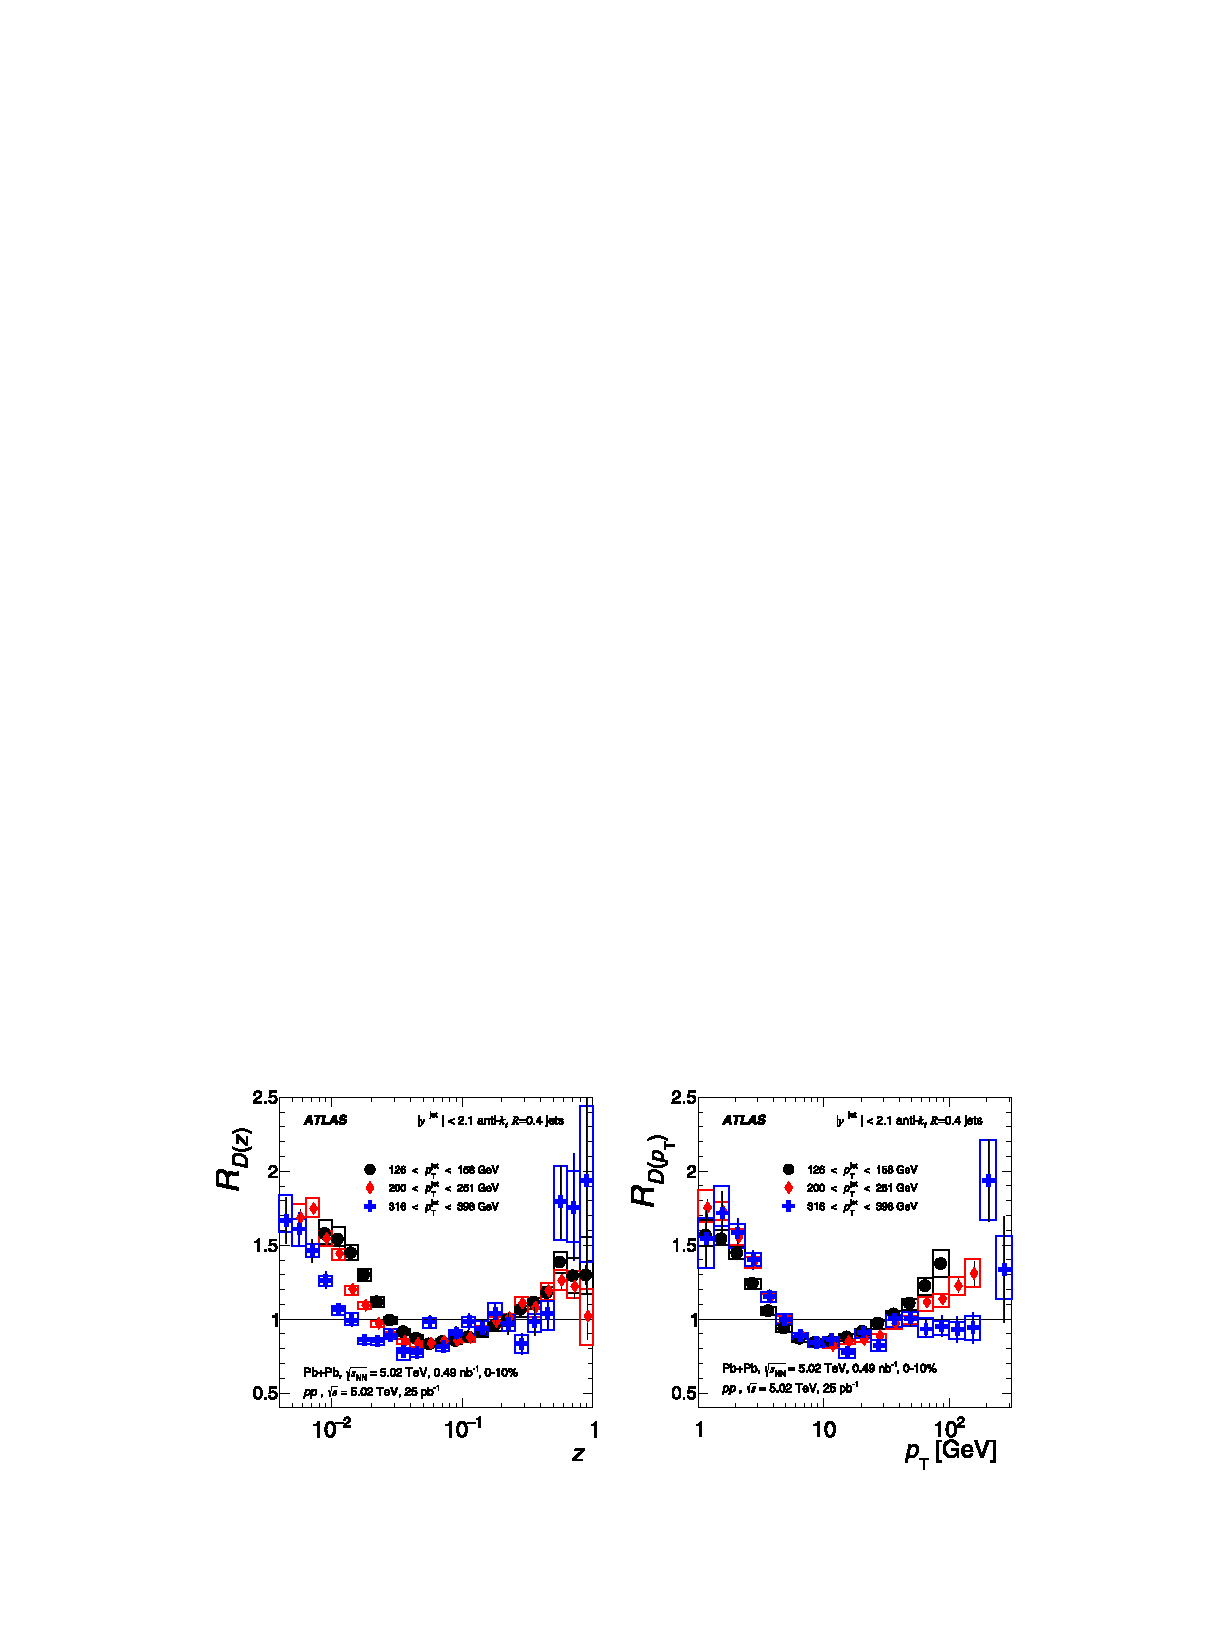
\includegraphics[width=0.75\textwidth]{figures/jetMeasurements/jetff_jetpt_dep}
%\caption{The \ptjet\ dependence of the \Rdz\ (left) and \Rdpt\ (right) distributions in 0--10\% central \pbpb\ compared to \pp\ collisions.
%The error bars represent statistical uncertainties while the shaded boxes represent systematic uncertainties.
%Figure taken from \cite{PhysRevC.98.024908}.}
%\label{fig:jetff_jetpt_dep}
%\end{center}
%\end{figure}


\begin{figure}[htbp]
\begin{center}
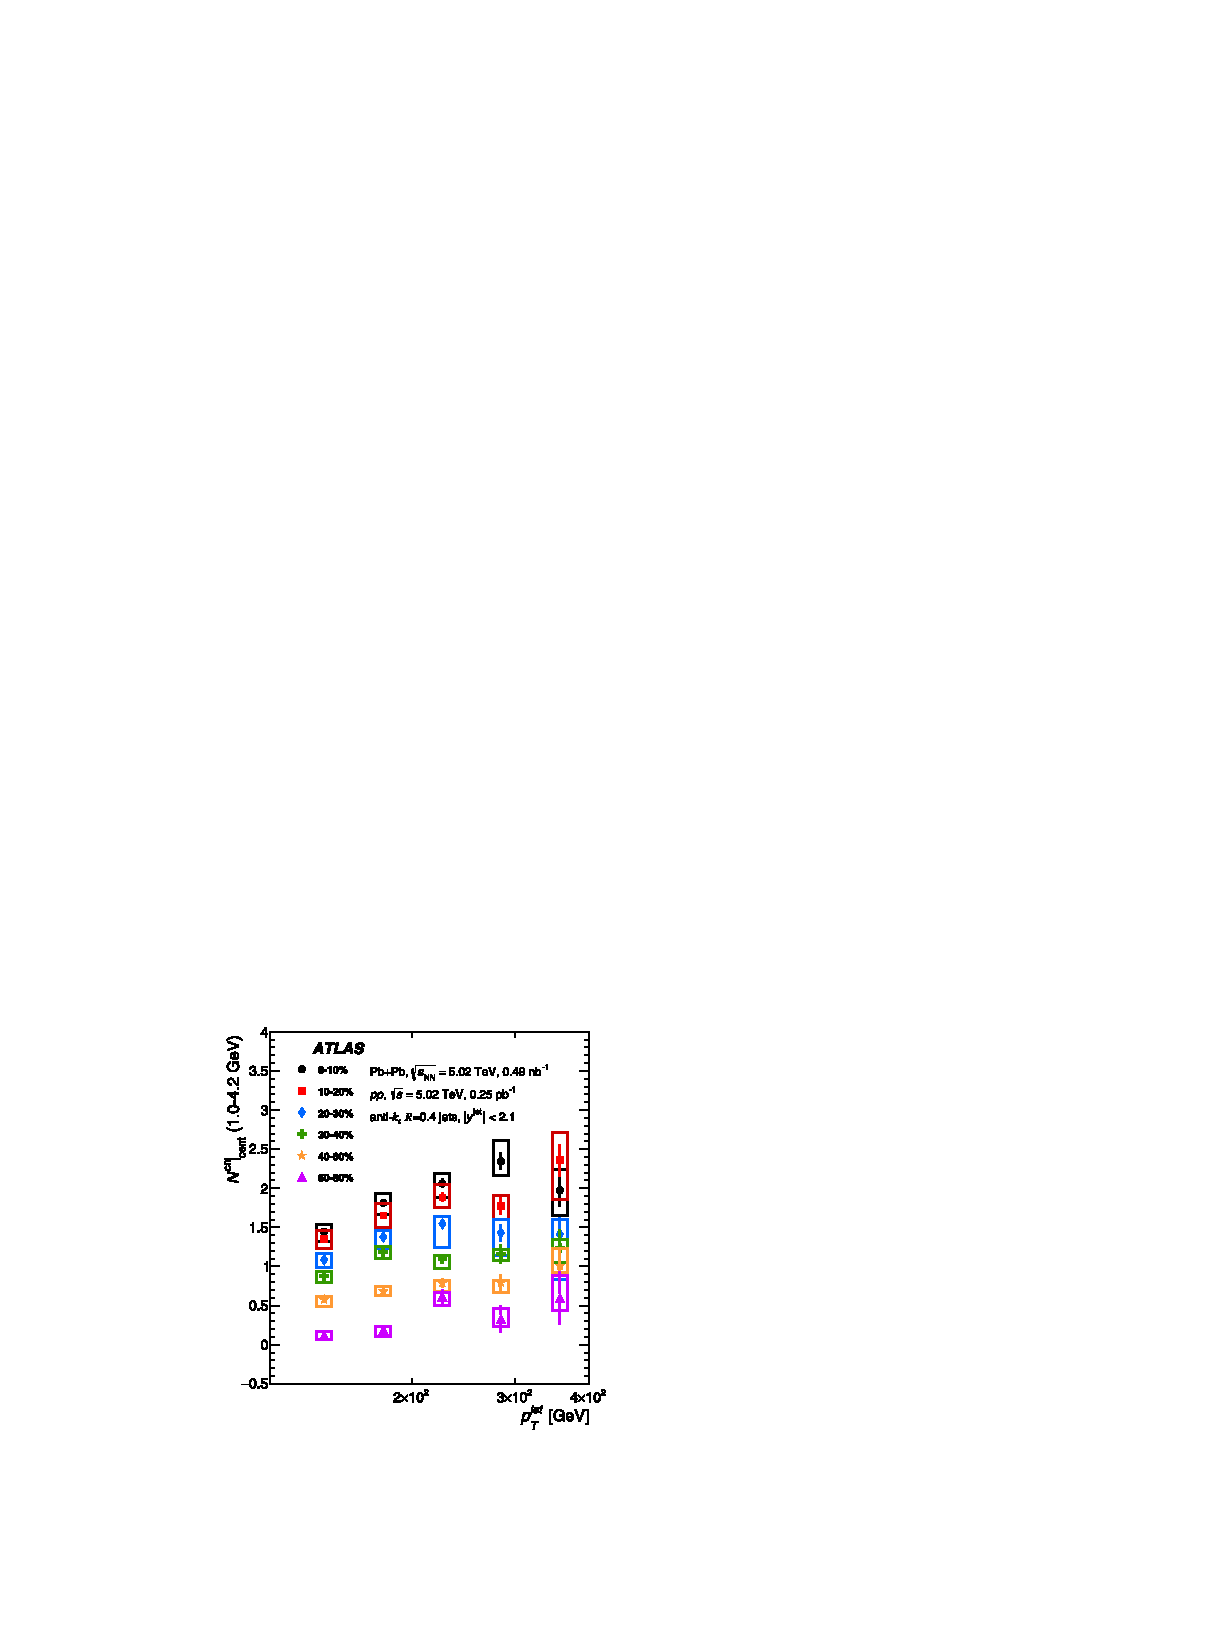
\includegraphics[width=0.35\textwidth]{figures/jetMeasurements/jetff_nch}
\caption{The number of extra particles that carry $1<\pt<4$ GeV  in \pbpb\ compared to \pp.
The different colors represent different centrality selections.
The error bars represent statistical uncertainties while the shaded boxes represent systematic uncertainties.
Figure taken from \cite{PhysRevC.98.024908}.}
\label{fig:jetff_nch}
\end{center}
\end{figure}

The modifications to the \Dz\ distributions have also been compared to a variety of models, including the Effective Quenching model \cite{Spousta:2015fca}, the Soft Collinear Effective Theory \cite{Chien:2015vja, Kang:2017frl}, and the Hybrid Model \cite{Casalderrey-Solana:2014bpa}.
These comparisons are shown in Figure~\ref{fig:jetff_rdz_theory}, and are discussed in detail in Chapter~\ref{sec:jetModels}.

\begin{figure}[htbp]
\begin{center}
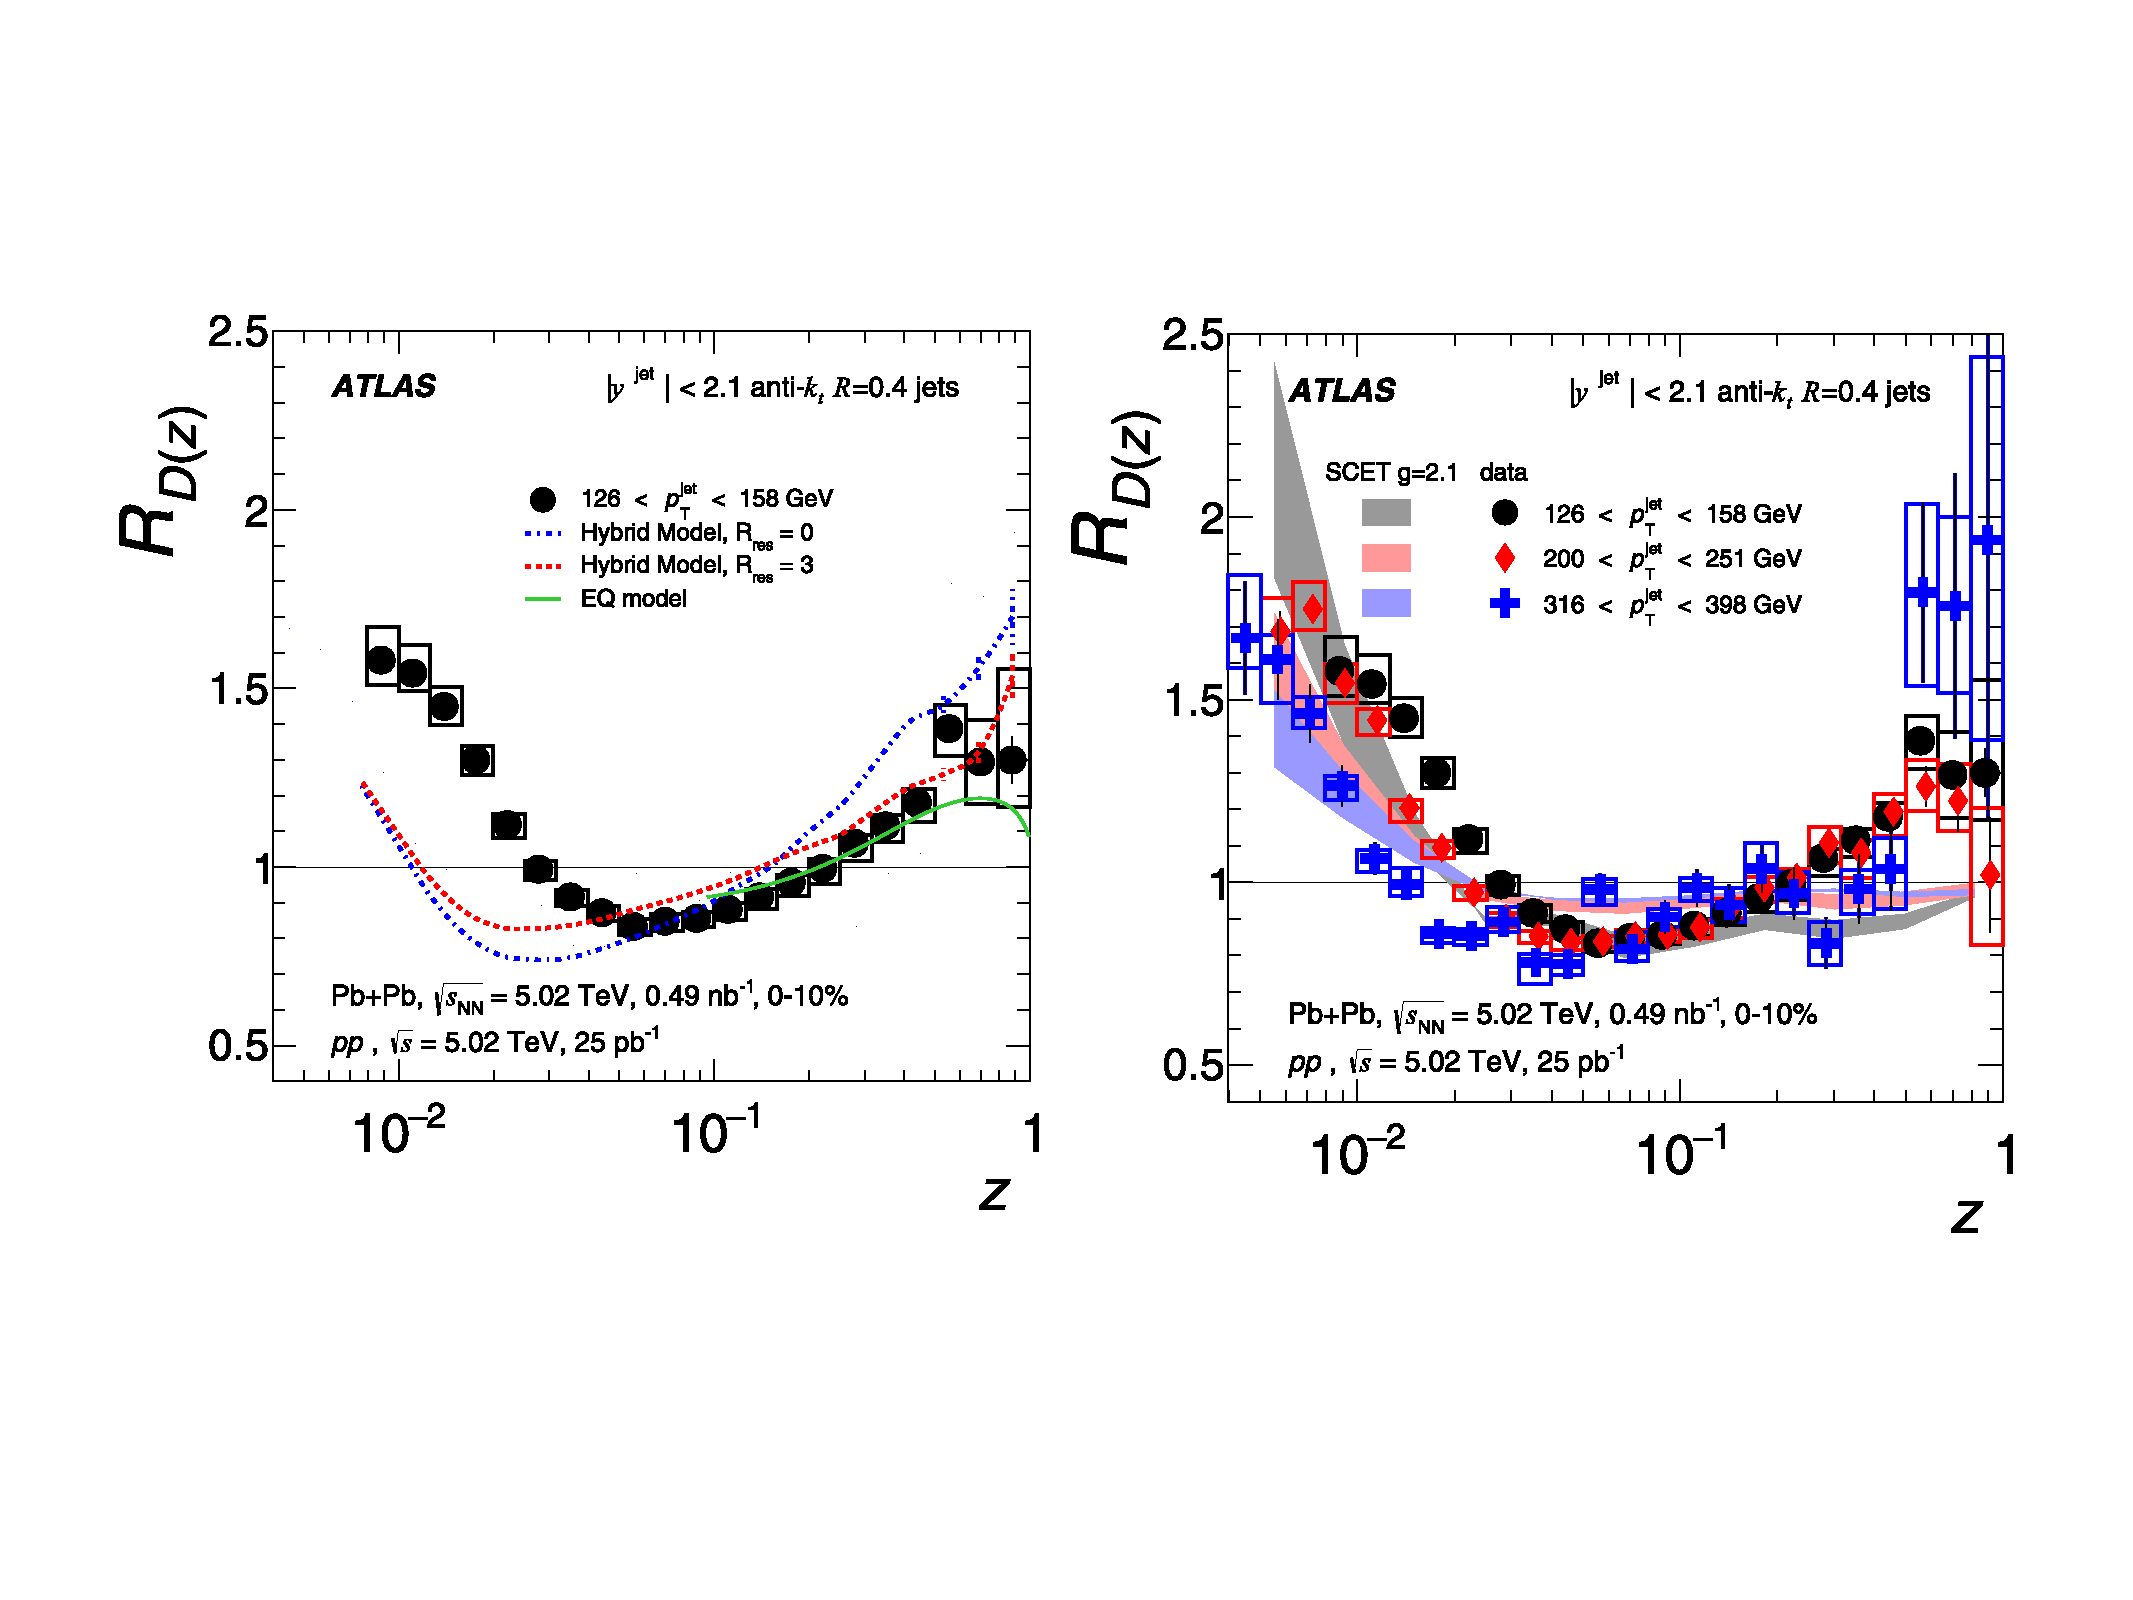
\includegraphics[width=0.75\textwidth]{figures/jetMeasurements/jetff_rdz_theory}
\caption{The \Rdz\ distributions compared to the EQ and Hybrid models (left) and SCET (right).
The error bars represent statistical uncertainties while the shaded boxes represent systematic uncertainties.
Figure taken from \cite{PhysRevC.98.024908}.}
\label{fig:jetff_rdz_theory}
\end{center}
\end{figure}



